\chapter{Introduction}
\label{sec:intro}
\chaptermark{Theoretical Motivation}
Modern particle physics is described by a theory called the standard model (SM).  
The SM describes a universe in which matter consists of particles of half-integer spin\footnote{Intrinsic angular momentum} called fermions.  
These fermions interact with each other through force mediating integer spin particles called bosons.  
This section will provide a basic outline of this theory as well as the known issues and need for a more basic theory.

\section{Fundamental Particles}
The SM matter in the universe is around 98\% Hydrogen and Helium with the final 2\% being heavier elements.  
To a very good approximation, the known matter in the universe consists of protons, neutrons, and electrons.  
Electrons are categorized in the standard model as leptons and are fundamental.  
Protons and neutrons are composites of three quarks.  
The up quark (u) has +2/3e\footnote{e is the magnitude of the charge of the electron} charge, and the down quark (d) has -1/3e charge, so the proton is an up-up-down combination and the neutron is down-down-up.  
These quark compounds are called hadrons and are categorized into two families: baryons (three quarks), and mesons (two quarks).

Although this is a good approximation of the known universe, through experimental and theoretical advances we know that there are 
more exotic phenomena that can be described by extending the known quarks and leptons to three generations.  
The three lepton generations are defined by the electron, muon, tau and their corresponding neutrinos.
The +2/3e charge quarks are the up, charm, and top; whereas the -1/3e charge quarks are the down, strange, and bottom.  
These quarks and leptons are summarized in Table~\ref{table:SMferm} along with their charge and mass.
    
Quarks and leptons define all known fermionic matter, with gauge boson particles being responsible for particle interactions.  
The final particle, the Higgs boson, is responsible for the mechanism by which particles acquire mass.  
    

\begin{table}[h]
\begin{center}
\begin{tabular}{l|c|c}
\hline
\hline
particle & charge (e) & mass (MeV)\\ \hline \hline
e & -1 & 0.5110 \\
$\mu$ & -1 & 105.7\\
$\tau$ & -1 & 1777\\
$\nu_{\mathrm{e}}$, $\nu_{\mu}$, $\nu_{\tau}$ & 0 & $<$ 2 $\times \mathrm{10^{-6}}$ \\
u & +2/3 & 2.3\\
d & -1/3 & 4.8\\
s & -1/3 & 95\\
c & +2/3 & 1.275 $\times \mathrm{10^3}$ \\
b & -1/3 & 4.18 $\times \mathrm{10^3}$\\
t & +2/3 & 173.2 $\times \mathrm{10^3}$\\
\hline
\end{tabular}
\end{center}
\caption{List of SM fermions with their charge and mass.  These particles all have spin 1/2~\cite{PDG-2014}.}
\label{table:SMferm}
\end{table}


\section{Fundamental Interactions}
Interactions in the SM can be described by the four fundamental forces: electromagnetic, weak nuclear, strong nuclear, and gravity.  
These forces manifest by the exchange of a corresponding elementary boson.  
The intrinsic properties of these force carrying particles are responsible for the range and relative strength of the interaction.


The electromagnetic force is responsible for well known phenomena such as molecular bonds.  
This force is mediated be the photon, a massless, chargeless, spin 1 particle, which photon interacts with charged particles only.        
The fact that the photon is massless leads to the infinite range of the electromagnetic force.  


The weak nuclear force manifests itself in nuclear decay, and is described by three force carrying bosons; the $\mathrm{W^+}$,$\mathrm{W^-}$, and Z.  
These bosons are massive, which leads to the weak force being short range.  
The $\mathrm{W^{\pm}}$ bosons have a charge of $\pm$e   whereas the Z boson is chargeless, and all three have spin 1.  
The weak force is responsible for transitions between flavors\footnote{The six quark types} of quarks (see Section~\ref{sec:weaktheory}).
Quarks and leptons both interact by the weak force.


The strong nuclear force is responsible for binding quarks together to form hadrons.  
The strong force describes the interactions of particles that carry color.  
Color is an intrinsic property of fundamental particles, and has three varieties; red, green and blue.
This force is mediated by gluons, which are massless and interact with quarks.  
The strong force is the strongest and shortest range of the known forces.  
The theory behind the strong force is described in more detail in Section~\ref{sec:qcdtheory}

The fourth known force, gravity, is both the most recognizable and least understood of the forces.  
All attempts at including gravity into the SM have failed, but hypothetically gravity should be mediated by the spin 2 graviton, which interacts with massive particles..
Gravity is by far the weakest of the fundamental forces. 

The force carrying bosons and their properties are listed in table \ref{table:SMbos}


\begin{table}
\begin{center}
\begin{tabular}{l|c|c|c}
\hline
\hline
particle & charge (e) & spin & mass (GeV)\\ \hline \hline
$\gamma$  & 0 & 1 & 0\\ 
$\mathrm{W^{\pm}}$ & $\pm$1 & 1 & 80.4\\
Z & 0 & 1 & 91.2\\ 
gl & 0 & 1 & 0 \\ 
gr & 0 & 2 & $<$ 6 $\times$ $\mathrm{10^{-38}}$ \\ 
\hline
\end{tabular}
\end{center}
\caption{List of SM force carrying bosons with their charge, mass and spin.  The graviton has not yet been observed~\cite{PDG-2014}.}
\label{table:SMbos}
\end{table}


\section{Feynman Diagrams}
Calculations in theoretical particle physics are facilitated by the use of Feynman diagrams.  
Feynman diagrams are pictorial representations that aid in the calculation of physical observables.  
These diagrams include the particles that interact (external lines), as well as the particles that mediate the interaction (internal lines), 
and where these external and internal lines intersect (vertices).  
An example diagram is shown in Figure~\ref{figs:emuScattering}.  
In this diagram, an electron and a positron\footnote{Shown as an electron with an inverted line direction} interact with a photon ($\gamma$), and a force is observed.
This diagram represents Bhabha scattering (responsible for electromagnetic attraction).  

\begin{figure}
\begin{center}
\unitlength=1mm
\begin{fmffile}{feynman/emuScattering}
\begin{fmfgraph*}(40,30) \fmfpen{thick}
\fmfleft{i1,i2} \fmfright{sp1,sp2}
\fmf{fermion}{i1,v1,sp1}
\fmf{fermion}{sp2,v2,i2}
\fmf{photon,label=$\gamma$}{v1,v2}
\fmflabel{$e^-$}{i1}
\fmflabel{$e^-$}{i2}
\fmflabel{$e^-$}{sp1}
\fmflabel{$e^-$}{sp2}
\end{fmfgraph*}
\end{fmffile}
\end{center}
\caption{Feynman diagram depicting electron-positron scattering via
the electromagnetic interaction.}
\label{figs:emuScattering}
\end{figure}


The rules governing the calculation of physical observables from these diagrams are defined by the theory of Quantum Electrodynamics (QED).
Using these diagrams, the rules of QED let us calculate the matrix element ($\cal{M}$).  

$\cal{M}$ can by related to physical quantities through the square modulus ($|\cal{M}|^{\mathrm{2}}$), which is the probability density for a process to occur.   
From this, relevant quantities such as the cross section (see Section~\ref{sec:LumiXsec}) of the process can be calculated.  

Additionally, in the case that a particle decays we can evaluate the decay width ($\Gamma$).  
When a particle of mass M decays, there is a range of observed values of mass following a Breit-Wigner distribution centered at M.
The decay width represents the width of this distribution at half the maximum.  The average lifetime of the particle is 1/$\Gamma$.  

For a given process there can be multiple contributing diagrams, for instance for a calculation involving the Coulomb attraction shown in Figure~\ref{figs:emuScattering}, 
one must also consider the 
diagram shown in Figure~\ref{figs:emuScattering2}, which has the same incoming and outgoing particles.  
Diagrams such as this interfere with each other constructively or destructively in the calculation of the matrix element, 
which can increase or decrease the cross section of the full process.  

\begin{figure}
\begin{center}
\unitlength=1mm
\begin{fmffile}{feynman/emuScattering2}
\begin{fmfgraph*}(40,30) \fmfpen{thick}
\fmfleft{i1,i2} \fmfright{sp1,sp2}
\fmf{fermion}{i1,v1,i2}
\fmf{fermion}{sp2,v2,sp1}
\fmf{photon,label=$\gamma$}{v1,v2}

\fmflabel{$e^-$}{i1}
\fmflabel{$e^-$}{i2}
\fmflabel{$e^-$}{sp1}
\fmflabel{$e^-$}{sp2}


\end{fmfgraph*}
\end{fmffile}

\end{center}
\caption{Feynman diagram depicting electron-positron scattering via
the electromagnetic interaction in the s channel.}
\label{figs:emuScattering2}
\end{figure}


Vertices in a Feynman diagram are points where energy and momentum are conserved in the calculation.  
Each of the vertices contributes a factor of the coupling constant $\alpha$ to the matrix element computation.  
In the calculation of the full matrix element for the electron positron scattering shown in Figures~\ref{figs:emuScattering} and~\ref{figs:emuScattering2}, 
we must consider diagrams with higher vertex multiplicity such as those seen in Figure~\ref{figs:emuScatteringnlo2}.  
To approximate $\cal{M}$ in QED, we can perform an expansion in the vertex multiplicity n, summing over matrix elements within the same order i ($\cal{M}_{\mathrm{i}}^{\mathrm{n}}$). 
 .  

\begin{figure}
\begin{center}
\unitlength=1mm
\begin{fmffile}{feynman/emuScatteringnlo1}
\begin{fmfgraph*}(40,30) \fmfpen{thick}
\fmfleft{i1,i2} \fmfright{sp1,sp2}
\fmf{fermion,tension=1.5}{i1,m1,v1,m2,i2}
\fmf{fermion}{sp2,v2,sp1}
\fmf{photon,label=$\gamma$}{v1,v2}
\fmf{photon,tension=0.0,left}{m1,m2}
\fmflabel{$e^-$}{i1}
\fmflabel{$e^-$}{i2}
\fmflabel{$e^-$}{sp1}
\fmflabel{$e^-$}{sp2}
\end{fmfgraph*}
\end{fmffile}
\end{center}
%\caption{Feynman diagram depicting NLO electron-positron scattering via
%the electromagnetic interaction.}
%\label{figs:emuScatteringnlo1}
\end{figure}

\begin{figure}
\begin{center}
\unitlength=1mm
\begin{fmffile}{feynman/emuScatteringnlo2}
\begin{fmfgraph*}(40,30) \fmfpen{thick}
\fmfleft{i1,i2} \fmfright{sp1,sp2}
\fmf{fermion}{i1,v1,i2}
\fmf{fermion}{sp2,v4,sp1}
\fmf{photon}{v1,v2}
\fmf{fermion,tension=0.5,left}{v2,v3,v2}
\fmf{photon}{v3,v4}
\fmflabel{$e^-$}{i1}
\fmflabel{$e^-$}{i2}
\fmflabel{$e^-$}{sp1}
\fmflabel{$e^-$}{sp2}
\end{fmfgraph*}
\end{fmffile}
\end{center}
\caption{Feynman diagram depicting NLO electron-positron scattering.}
\label{figs:emuScatteringnlo2}
\end{figure}


\begin{eqnarray}
\cal{M} = \sum\limits_{\mathrm{n=1}}^\infty \sum\limits_{\mathrm{i}}  \cal{M}_{\mathrm{i}}^{\mathrm{n}}
\label{eqn:matrixelement}
\end{eqnarray}  

Due to the fact that the coupling constant in QED is 1/137, this expansion can terminate quickly because high n diagrams contribute much less to $\cal{M}$.  
A calculation involving all diagrams with the least number of vertices is called leading order.  
Calculations involving all diagrams with higher order contributions as well are called next-to leading order (NLO), next-to-next-to leading order (NNLO), etc.    

Once the matrix element has been determined to an acceptable accuracy, we can extract the cross section in a straight forward manner.  
For the example electron-positron scattering process above the differential cross section has the following simplified equation due to the special case of identical mass particles:  

\begin{eqnarray}
\left(\frac{\mathrm{d\sigma}}{\mathrm{d\Omega}}\right)_{\mathrm{CM}} = \mathrm{\frac{|\cal{M}|^{\mathrm{2}}}{64 \pi^{2} E_{cm}^{2}}}
\label{eqn:xsecfromsigma}
\end{eqnarray}  


\section{Quantum Chromodynamics}
\label{sec:qcdtheory}
Quantum chromodynamics (QCD) is the theory describing the strong force, and is of particular importance for this thesis.  
The strong force is mediated by gluons which interact with particles that carry color.  
In QED, the photon is not charged, and thus can not interact with itself, however in QCD the gluon carries color and thus can interact with itself.  
Additionally, whereas the addition of a vertex greatly reduces the cross section in QED, the strong coupling constant $\alpha_s$ is of order 1, so 
higher order diagrams can contribute substantially to the measurement.  This means that QCD processes are much more difficult to calculate than QED 
processes.

However, $\alpha_s$ is not constant, and in fact increases as the distance scale of an interaction increases (see Figure~\ref{figs:alphasrunning}).  
This property of the the strong interaction is called asymptotic freedom.  For high $|q^2|$, $\alpha_s$ has the following form:

\begin{eqnarray}
\mathrm{\alpha_{s}(|q^2|)} =  \frac{\mathrm{\alpha_{s}(\mu^{2})}}{\mathrm{1+(\alpha_{s}(\mu^{2})/12\pi)(11n-2f)ln(|q^2|/\mu^{2})}}
\label{eqn:qcdalphas}
\end{eqnarray}  
%from Griffiths

where n is the number of colors (3), and f is the number of flavors (6), and $\mu^{2}$ is some arbitrary energy where $\alpha_{s}(\mu^{2})$ $<$ 1.
Therefore because 11n $>$ 2f, $\alpha_{s}$ will decrease as energy increases.


Therefore as the distance between two quarks increases, so do the forces holding them together.  
This large force at a characteristic distance ($\sim10^{-15}$ m) is the reason why it is difficult to observe a free quark (quark confinement).  
Although quarks can not be observed alone, there are ways of precisely determining the physical properties of free quarks through reconstruction of their decay products.  




\begin{figure}
\begin{center}
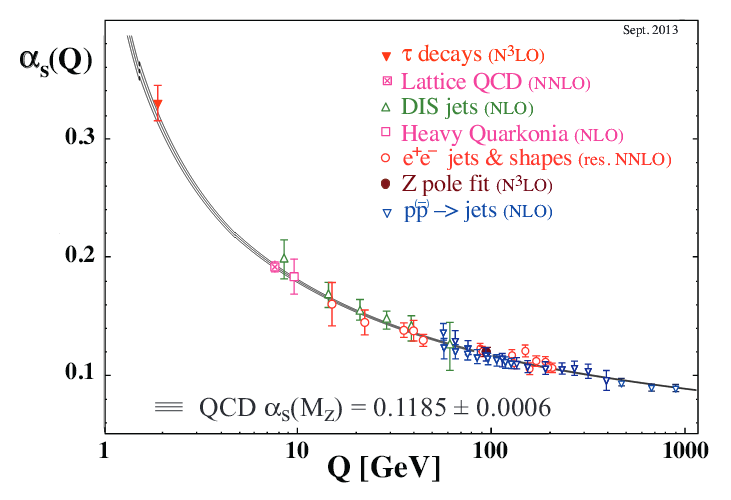
\includegraphics[width=1.0\linewidth]{figs/alphasrunning.png}
\caption{The QCD coupling constant $\alpha_{\mathrm{S}}$ as a function of the energy scale Q~\cite{PDG-2014}.}
\label{figs:alphasrunning}
\end{center}
\end{figure}
%from pdg


When a quark pair is produced with a high momentum, their separation increases quickly.  
As the separation of these quarks increases, the energy of the QCD field between them increases as well.  
If this separation is high enough, the energy between the quarks will reach a threshold where quark pair production is energetically favorable.  
At this threshold, the constituent quarks are then joined by these pair produced quarks.  
Additional quark pairs can be created many times, and the initial quark is detected as many hadrons that are collimated into a stream of particles called a jet.  
This process is called hadronization.  

The $\alpha_s$ parameter is low at short distances (or equivalently high energy); 
just like in QED, the impact of higher order diagrams is small.  
In this regime, QCD calculations using a finite expansion is possible which allows us to only consider free quarks. 
The characteristic interaction energy where free quarks can be considered is above the constant $\Lambda$, which is in the range of 100~$\MeV$ to 500~$\MeV$.
This is much lower than energy scales considered in this thesis, so we will only be referring to free quark interactions \cite{Griffiths}.  


\section{Parton Distribution Functions}
\label{sec:pdftheory}
Hadrons are composite objects made up of two or three ``valence'' quarks, but also contain quark-antiquark pairs (``sea quarks'') and gluons (see Figure~\ref{figs:partons}).  
These sea quarks and gluons are very important to consider when analyzing hadrons.  
Take for instance the quark masses listed in Table~\ref{table:SMferm}.  
Summing the valence quark mass for a proton, we would assume a proton would have a mass of 9.4$~\MeV$, but the proton has a measured mass of 938.3$~\MeV$.  

Therefore, the energy of a proton is shared among the partons, and for calculations it is useful to define parton distribution functions (PDFs). 
PDFs define the probability of a parton to carry a fraction x of the hadron.  
Figure~\ref{figs:pdfs} shows parton distribution functions for the proton at two characteristic energy scales.  


\begin{figure}
\begin{center}
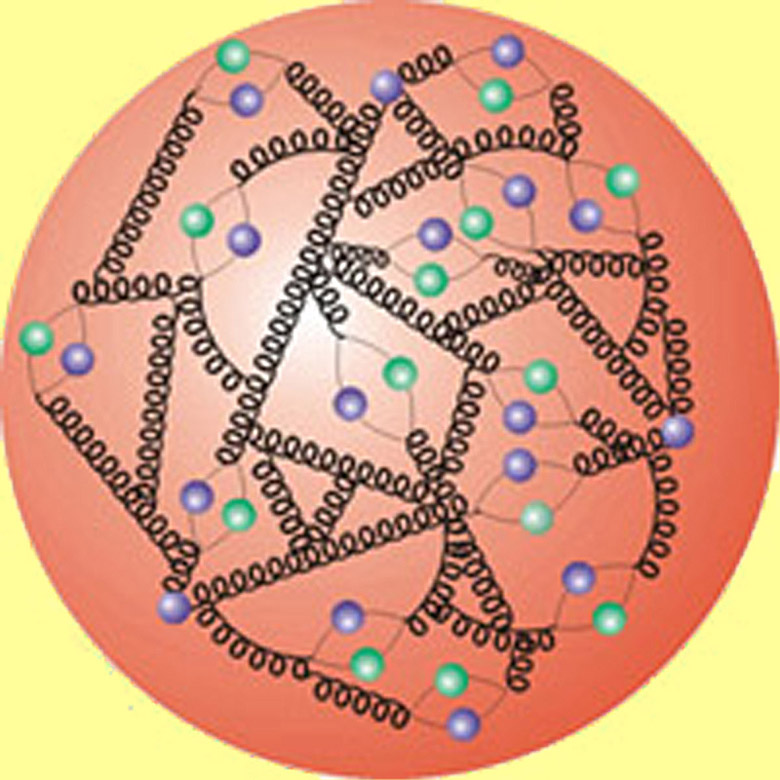
\includegraphics[width=0.4\linewidth]{figs/partons.jpg}
\caption{An illustration of a proton emphasizing the sea quark contribution~\cite{fnal}.}
\label{figs:partons}
\end{center}
\end{figure}
%fnal.gov

\begin{figure}
\begin{center}
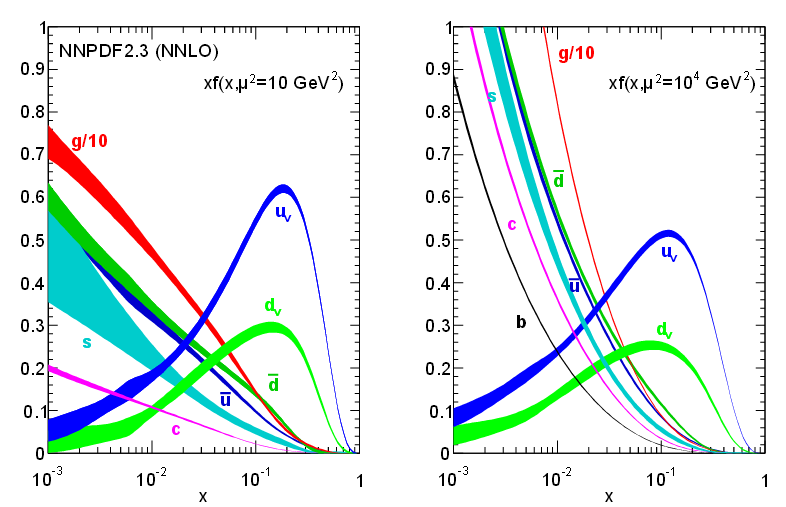
\includegraphics[width=.8\linewidth]{figs/pdfs.png}
\caption{Parton distrubution functions for the proton.  The left plot is evaluated at an energy scale of $\mathrm{\mu^{2}~=~10~\GeV^{2}}$, and the 
right plot at $\mathrm{\mu^{2}~=~10^{4}~\GeV^{2}}$~\cite{PDG-2014}.   }
\label{figs:pdfs}
\end{center}
\end{figure}
%pdg


\section{The Weak Force}
\label{sec:weaktheory}
The weak force is felt by both quarks and leptons.  
It is weaker than both the electromagnetic and the strong force, which leads to longer decay times for weakly decaying particles.  
The weak force is responsible for changing of quark flavor in an interaction.  
A vertex involving a change is quark flavor contributes a factor of $\mathrm{V_{ij}}$ to the matrix element, where $\mathrm{V_{ij}}$ is an element of the Cabibbo Kobayashi Maskawa (CKM) matrix 
(shown in Figure\ref{figs:CKM}).  
For example, the calculation of the diagram in Figure~\ref{figs:betaDecay} (beta decay) includes a factor of $\mathrm{V_{ud}}$ = 0.97427.  
The CKM matrix is roughly diagonal, which means that a process which changes quark generation is rare.  

\begin{figure}
\begin{center}
\unitlength=1mm
\begin{fmffile}{feynman/betaDecay}
\begin{fmfgraph*}(40,30) \fmfpen{thick}
\fmfleft{i1,i2} \fmfright{sp1,sp2,sp3}
\fmf{phantom}{i2,v2,sp3}
\fmf{fermion}{i1,v1,sp1}
\fmf{fermion,tension=0.0}{v2,sp2}
\fmf{fermion,tension=0.0}{sp3,v2}
\fmf{photon,label=$W^{-}$}{v1,v2}
\fmflabel{$d$}{i1}
\fmflabel{$u$}{sp1}
\fmflabel{$e^-$}{sp2}
\fmflabel{$\nu_{e}$}{sp3}
\end{fmfgraph*}
\end{fmffile}
\end{center}
\caption{Feynman diagram depicting beta decay via
the weak interaction.}
\label{figs:betaDecay}
\end{figure}


Weak force interactions are dependent on the chirality of the interacting particle.
Chirality for massless particles is dependent on the relative orientation of the momentum and spin axes.  
Particles with momentum and spin aligned are referred to as right-handed, and particles with the momentum 
axis opposite to spin are left-handed\footnote{This convention is reversed for anti-particles}.
For massive particles this concept is generalized such that right- and left-handed components of a wavefunction 
can be extracted by using the right-handed operator (1+$\gamma^5$)/2 and the left-handed operator (1-$\gamma^5$)/2.  
The W boson only interacts with left-handed fermions whereas the Z boson interacts with right- and left-handed fermions with differing strengths. 

\begin{figure}
\begin{center}
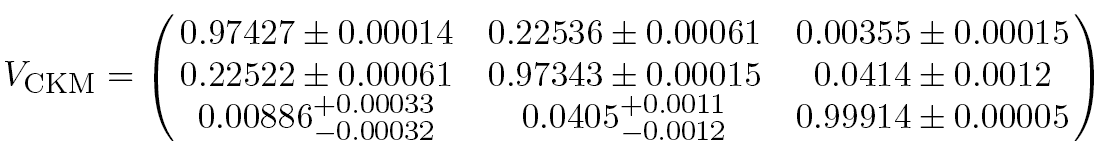
\includegraphics[width=1.0\linewidth]{figs/CKM.png}
\caption{The CKM quark mixing matrix~\cite{PDG-2014}.}
\label{figs:CKM}
\end{center}
\end{figure}



\section{Electroweak Symmetry Breaking}
%From pdg
Through the electroweak symmetry breaking mechanism, the mass of the W and Z bosons, and all fermions can be generated in the SM.  
We consider a scalar potential of the form:
\begin{eqnarray}
\mathrm{ V(\Phi) = m^{2} \Phi^{\dagger} \Phi + \lambda ( \Phi^{\dagger} \Phi )^{2}  }\\
\mathrm{\Phi = \frac{1}{\sqrt{2}} \left( \frac{\sqrt{2} \phi^{+}}{\phi^{0} + ia^{0}}  \right)}
\end{eqnarray}  
where $\Phi$ is the Higgs field.  A plot of this potential can be seen in Figure~\ref{figs:higgspotential}.  
The minimum of the potential is not at V(0), and this point is unstable.  
The Higgs field has a non-zero vacuum expectation value (VEV).

\begin{figure}
\begin{center}
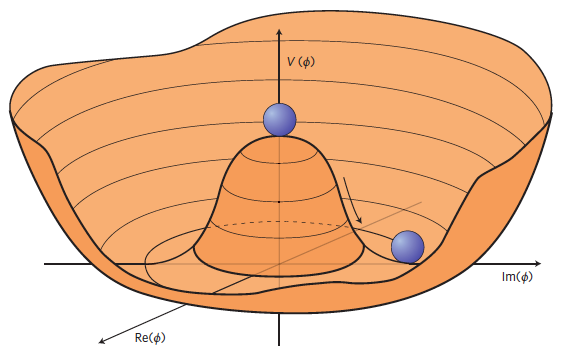
\includegraphics[width=0.7\linewidth]{figs/higgspotential.png}
\caption{The Higgs potential..}
\label{figs:higgspotential}
\end{center}
\end{figure}

Using the Higgs Lagrangian
\begin{eqnarray}
\cal{L} = \mathrm{(D_{\mu} \Phi )^{\dagger}(D_{\mu} \Phi ) -V( \Phi )}\\
\mathrm{(D_{\mu}\Phi) = (\partial_{\mu}+i g \sigma^{\alpha} W_{\mu}^{\alpha}/2 +i g^{'} Y B_{\mu}/2)\Phi}
\end{eqnarray}  
we can extract the masses of the W and Z bosons as

\begin{eqnarray}
M_{W}^2 = \frac{g^{2}v^{2}}{4}\\
M_{Z}^2 = \frac{(g^{'2}+g^{2})v^{2}}{4}
\end{eqnarray}  

One new particle is predicted, a massive, chargeless, spin 0 boson called the Higgs.  
A particle consistent with the Higgs boson has been discovered in 2012 at the LHC.  
%https://cds.cern.ch/record/1638469/plots

  
\section{Beyond the Standard Model}
\label{sec:BSMtheory}
The SM is possibly the most successful theory in physics, but also one that is ultimately incomplete.  
We know that there are physical phenomena that the SM does not predict.  
The presence of dark matter and dark energy in the universe~\cite{Bennett:2003ba} is not currently explained by the SM.  
Given that dark matter and energy account for approximately 95\% of the universe, this is not a small issue.  
The SM does not explain the observation of neutrino oscillations~\cite{An:2012eh}, which implies that neutrinos have mass.  
The SM also does not naturally explain the relative values of fundamental constants such as why the weak force is $10^{29}$ times as strong as gravity.  
This issue is known as the hierarchy problem, and it is assumed that a complete theory would have a natural explanation for the seemingly random values of these constants.  

It is essential for a complete understanding of the universe that we probe beyond the standard model (BSM) theories that provide solutions to these issues.  
Theories involving compact extra dimensions~\cite{PhysRevD.64.035002} for example provide a natural explanation to the hierarchy problem.  
In these theories forces propagate in higher dimensions that are compactified.   
In this theory, the propagation of SM massive fields in higher dimensions leads to discrete modes, which are detectable as new massive particles.  
The propagation of the SM W or Z leads to excited modes that are referred to as the $\wpr$ and $\zpr$.
A novel way to look for BSM physics then is to attempt the creation and detection of massive states such as these bosons. 
In this thesis we discuss one such search for a W' boson, which is additionally predicted by many BSM theories such as Little Higgs~\cite{doi:10.1146/annurev.nucl.55.090704.151502}, 
Composite Higgs models~\cite{Vecchi:2013bja}, and Noncommuting Extended Technicolor~\cite{Chivukula:1995gu}.  



